\documentclass{article}

\usepackage{tikz}
\usetikzlibrary{positioning, fit,  shapes.geometric}
\usepackage{ifthen}
\usepackage{etoolbox}

\tikzset{
	backgroundcolor/.style ={fill=white},
	every node/.append style={
		minimum height=7mm,
	},
	labe/.append style={
		%Blue,
		align = center,
		backgroundcolor,
		fill opacity=0.6,
		text opacity=1,
		font={\footnotesize\itshape}	
	},
	layer/.append style={
		draw,
		align = center,
		minimum height=7mm,
	},
	tight/.append style={
		inner sep=0.2mm,
	},
	lookupbox/.append style={
		draw=none,
		append after command={
		       	[shorten <= -0.5\pgflinewidth]
		       	([shift={(-1.5\pgflinewidth,-0.5\pgflinewidth)}]\tikzlastnode.north east)
		       	edge([shift={( 0.5\pgflinewidth,-0.5\pgflinewidth)}]\tikzlastnode.north west) 
		       	([shift={( 0.5\pgflinewidth,-0.5\pgflinewidth)}]\tikzlastnode.north west)
		       	edge([shift={( 0.5\pgflinewidth,-1.5\pgflinewidth)}]\tikzlastnode.south west)            
		       	([shift={( -1.5\pgflinewidth,+0.5\pgflinewidth)}]\tikzlastnode.south east)
		       	edge([shift={(-1.5\pgflinewidth,-0.5\pgflinewidth)}]\tikzlastnode.north east)
		},
		inner sep=0.7mm,
		outer sep=0mm,
		minimum width=25mm
	}
}

\begin{document}

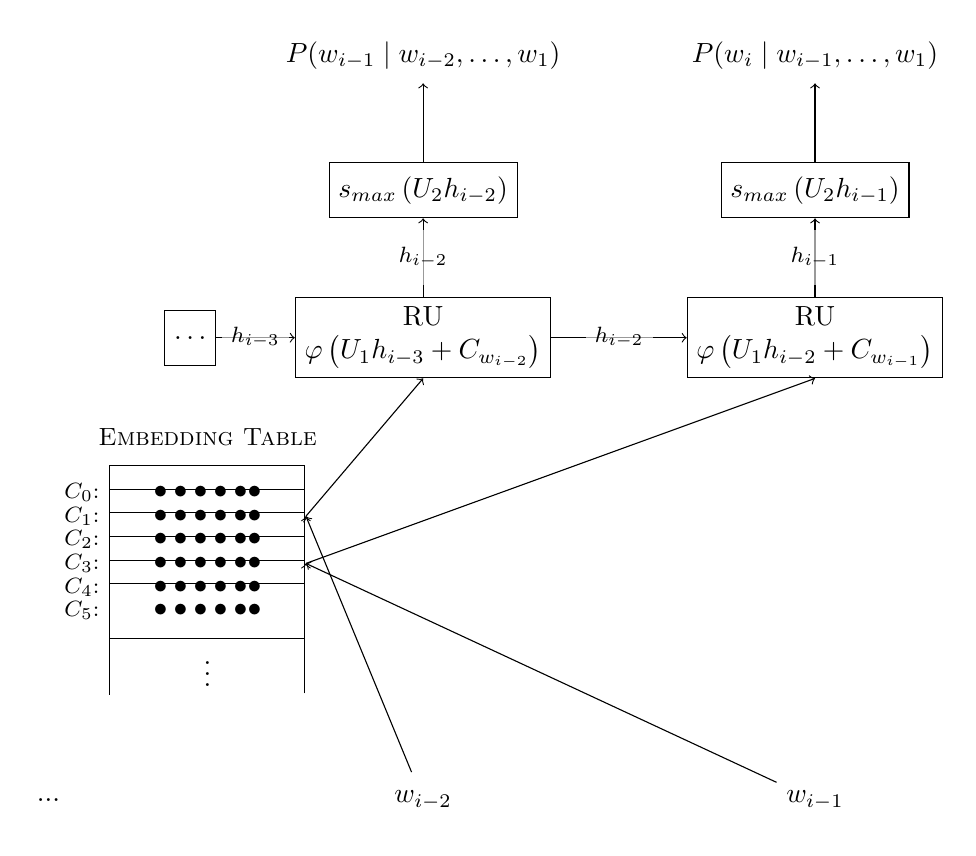
\begin{tikzpicture}[]

\newcommand{\hsep}{4}
\newcommand{\vtablesep}{5}

\node(w1) {$w_{i-1}$};
\node(w2)[left = \hsep of w1] {$w_{i-2}$};
\node(w3)[left = \hsep of w2] {$...$};


\node(Cn)[lookupbox, above left=of w2] {$\vdots$};
\def\tblmax{6}
\foreach \ii in {1,...,\tblmax} {
	\pgfmathsetmacro\pos{(\ii - 1) * 3 };
	\pgfmathtruncatemacro\jj{(\tblmax -\ii)};
	
	\node(C\ii)[lookupbox, above = \pos mm of Cn]{$\bullet\bullet\bullet\bullet\bullet\bullet$};
	\node(Clbl\ii)[left = 0mm of C\ii]{\footnotesize $C_\jj$:};
};
\node(C)[above = 0mm of C\tblmax] {\small \textsc{Embedding Table}};

\node(L11)[layer, above = \vtablesep of w1]{RU\\$\varphi\left( U_1h_{i-2}  +  C_{w_{i-1}}\right)$};
\node(L21)[layer, above = of L11]{$s_{max}\left(U_2 h_{i-1}\right)$};
\draw[->]  (L11) edge node[labe]{$h_{i-1}$} (L21);
\node(out1)[above = of L21]{$P(w_i \mid w_{i-1}, \ldots,  w_1)$};
\draw[->] (L21) edge (out1);

\node(L12)[layer, above = \vtablesep of w2]{RU\\$\varphi\left( U_1h_{i-3}  +  C_{w_{i-2}}\right)$};
\node(L22)[layer, above = of L12]{$s_{max}\left(U_2 h_{i-2} \right)$};
\draw[->]  (L12) edge node[labe]{$h_{i-2}$} (L22);
\node(out2)[above = of L22]{$P(w_{i-1} \mid w_{i-2}, \ldots,  w_1)$};
\draw[->] (L22) edge (out2);
\draw[->]  (L12) edge node[labe]{$h_{i-2}$} (L11);

\node(L13)[layer, left = of L12] {$\ldots$};
\draw[->]  (L13) edge node[labe]{$h_{i-3}$} (L12);


\draw[->] (w1) edge (C3.east);
\draw[->]  (C3.east) edge (L11.south);
\draw[->] (w2) edge (C5.east);
\draw[->]  (C5.east) edge (L12.south);


\end{tikzpicture}

\end{document}